\documentclass[11pt]{article}
\usepackage[utf8]{inputenc}
\usepackage{amsmath}
\usepackage{amsfonts}
\usepackage{amssymb}
\usepackage{graphicx}
\usepackage[super]{nth}
\usepackage{amsthm}
\usepackage{bm}
\newtheorem{theorem}{Theorem}
\newtheorem{objective}{Objective}
\newtheorem{model}{Model}
\usepackage{xcolor}
\definecolor{light-gray}{gray}{0.95}
\newcommand{\code}[1]{\colorbox{light-gray}{\texttt{#1}}}
\usepackage{listings}
\usepackage{placeins}

\usepackage[authoryear]{natbib}


\makeatletter
\renewcommand{\maketitle}{
\begin{center}

\pagestyle{empty}

{\LARGE \bf \@title\par}
\vspace{1cm}

{\Large Marcel Gietzmann-Sanders, Michael Courtney, Andrew Seitz, Curry Cunningham}\\[1cm]

University of Alaska Fairbanks


\end{center}
}\makeatother


\title{Technique for Dimensionality Reduction in Decision Modeling}

\date{2024}
\setcounter{tocdepth}{2}
\begin{document}
\maketitle

\section*{Introduction}

\subsection*{Value of Probabilistic Modeling}

\section*{Theory}

Standard probabilistic deep learning networks are typically framed as a classification problem, using categorical cross-entropy as the loss function (\cite{durr}). Each output neuron represents a potential choice, with the model predicting the probability of each choice being correct based on this loss formulation. For these choices, we provide the network with features encapsulating the relevant information. Training is then comprised of providing a series such decisions. 

However, this formulation introduces a critical challenge: if there are $N$ features per choice and $M$ potential choices, the overall dimensionality of the input space becomes $N \cdot M$. Adding even a single feature increases the dimensionality by $M$ not just 1.

This growth poses a significant challenge due to the "curse of dimensionality", where the amount of data required to effectively train models grows exponentially with the dimensionality of the input space (CITE).

\subsection*{Log-Odds Modeling}

To address this issue, we propose an alternative framing. Instead of predicting the probabilities directly, we predict the log-odds $\phi_m$ for each choice and calculate the probability $p_m$ using the softmax function:

$$p_m = \frac{e^{\phi_m}}{\sum_{m=1}^{M}e^{\phi_m}}$$

This approach reduces the feature space dimensionality to $N$ and effectively increases the number of training examples by a factor of $M$.

We can implement this log-odds model using standard probabilistic deep learning techniques by replicating the log-odds computation across all $M$ choices. The outputs are fed into a softmax layer with $M$ units, where the layer's weights are set to the identity matrix and biases are set to zero. Using categorical cross-entropy as the loss function ensures compatibility with standard probabilistic deep learning while enabling us to train the log-odds weights and significantly reduce the problem's dimensionality.

\subsection*{Contrast Sampling}

As $M$ grows large, a practical issue arises: for each training example, most instances of the internal log-odds model would ideally report very low log-odds, resulting in low probabilities. Ideally, only one choice should produce $p_m=1$. This is analogous to a class imbalance problem, where the model becomes prone to predicting the most common class (CITE).

To address this, we balance the training data. Instead of presenting the model with full decisions containing all $M$ choices, we create training pairs, or contrasts, where each pair consists of one selected choice and one unselected choice. This approach is valid because the log-odds model focuses on the relative likelihood of choices, making the number of choices considered at any one time irrelevant.

The primary risk in using contrasts is introducing bias by disproportionately sampling certain combinations of choices. To mitigate this, we randomly sample pairs from each decision, ensure an equal number of contrasts per decision, and an equal number of decisions per individual. This preserves the balance across the training data and avoids skewing the model's predictions.

\section*{Application}

\subsection*{Data}

We consider a series of tracks from 111 Chinook salmon (\textit{Oncorhynchus tshawytscha}) caught and monitored between 2013 and 2022 (CITE). These tracks were obtained from pop-up satellite archival tags which collect temperature, light level, and depth information at specified (sub day) intervals. This data is then passed through a proprietary algorithm from Wildlife Computers to determine likely longitude and latitude during each day of of monitoring (\cite{PSAT}). \newline

Environmental data was derived from the Global Ocean Biogeochemistry Hindcast dataset (10.48670/moi-00019) and the Global Ocean Physics Reanalysis (10.48670/moi-00021) from the E.U. Copernicus Marine Service Information. Net primary production (mg/m3/day) and mixed layer thickness (m) were aggregated per Uber h3 resolution 4 cell in the Northern Pacific. 

\subsection*{Formulation}

The resolution 4 Uber h3 cell containing each salmon location was identified and then, assuming a maximum travel distance of 100km (centeroid to centeroid) all adjacent cells within the 100km were identified as choices (including the currently occupied cell). In general this represented $\sim 19$ choices per decision with the intention being to predict the probability of moving to any particular cell. Training data was derived by identifying the actual cell moved to. 

\subsection*{Features} 

Movement heading in radians and distance to the centroid of the choice cell were computed and then mixed layer thickness and net primary production were joined to the choices on cell and day.

Distance was normalized to a range of 0-1 by division by 100, while mixed layer thickness and net primary production were both log-scaled and then centered at zero. 

\subsection*{Contrast Sampling}

After inspecting the distribution of number of choices per salmon and number of choices per decision, we decided on random sampling (with replacement) 200 decisions per individual and 19 choices per decision. 

Over a test/validation/training split of 40, 71 this resulted in 345,800 contrasts of which 269,800 were used in training and the rest in validation. 

Note that only 14,200 training examples would've been available to a traditional probabilistic approach representing a large increase in the number of available training examples.   

\subsection*{Training}

Three sets models were trained, one including only distance, one with both distance and movement heading, and one with all four features. Note that while the feature dimensions of these models are 1, 2, and 4 respectively, given the maximum number of choices per decision seen was 33 they dimensionality of a standard probabilistic model would've been 33, 66, and 132 representing a large reduction in the dimensionality of our feature spaces. 

Architectures/hyperparameters for the log-odds component of the model were parametrized in the following ways:

\begin{center}
\begin{tabular}{| c | c |} 
\hline 
Component & Options \\
\hline
Layers & 3, 4 \\ 
Units per Layer & 24, 32 \\
Batch Size & 10000 \\
Learning Rate & 0.0005 \\
\hline
\end{tabular}
\end{center}

With 5 models trained for each combination. Models were trained in Keras using an Adam optimizer for 100 epochs. 

Models for each set of features we selected on the basis of the loss over the validation set of contrasts. 

\section*{Results}

In training the metric of interest is the contrasts normalized log probability (C-NLP) - the average log probability per contrast. For an equivalent metric over all of the decisions we also computed the average log probability per decision for each individual and then computed an average over those across individuals (in order to not favor individuals with many decisions). This is the D-NLP reported in the table below. 

\begin{center}
\begin{tabular}{| c | c | c | c | c |}
\hline 
Model & Train C-NLP & Val C-NLP & Train D-NLP & Val D-NLP \\
\hline
No Model & -0.693 & -0.693 & -2.944 & -2.944 \\
Model 1 & -0.172 & -0.154 & -1.336 & -1.223 \\
Model 2 & -0.156 & -0.150 & -1.281 & -1.200 \\
Model 3 & -0.147 & -0.146 & -1.248 & -1.180 \\
\hline
\end{tabular}
\end{center}

"No Model" assumes all decisions are equally likely, Model 1 is the distance only model, Model 2 adds the movement heading, and Model 3 adds the net productivity and mixed layer thickness features. \newline

\begin{figure}[h!] 
	\centering
  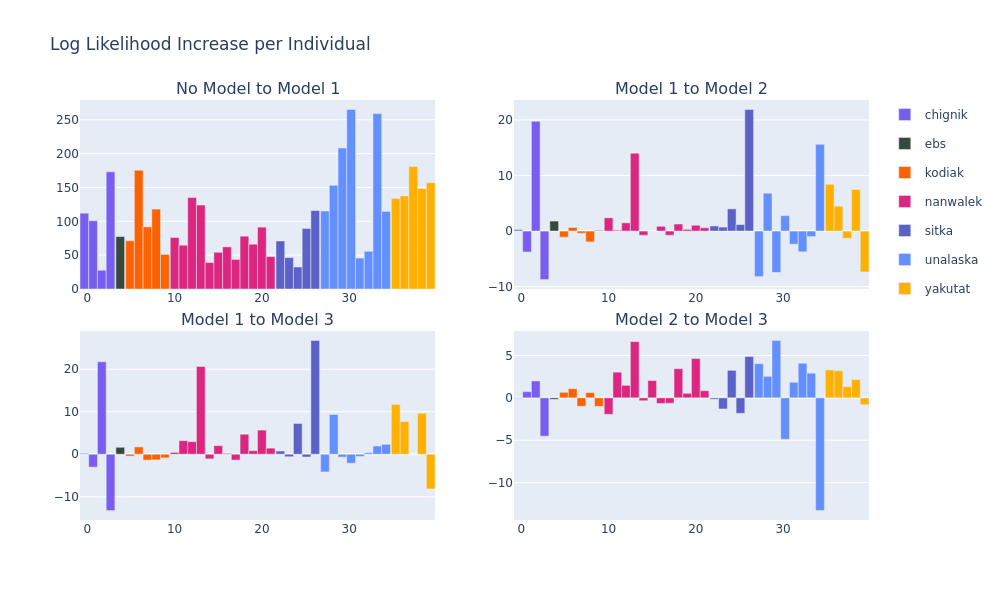
\includegraphics[height=70mm]{figures/ll_increase.png}
  \caption{Log likelihood increase (unnormalized) per individual of each model change.}
  \label{fig:ll_increase}
\end{figure}

\begin{figure}[h!] 
	\centering
  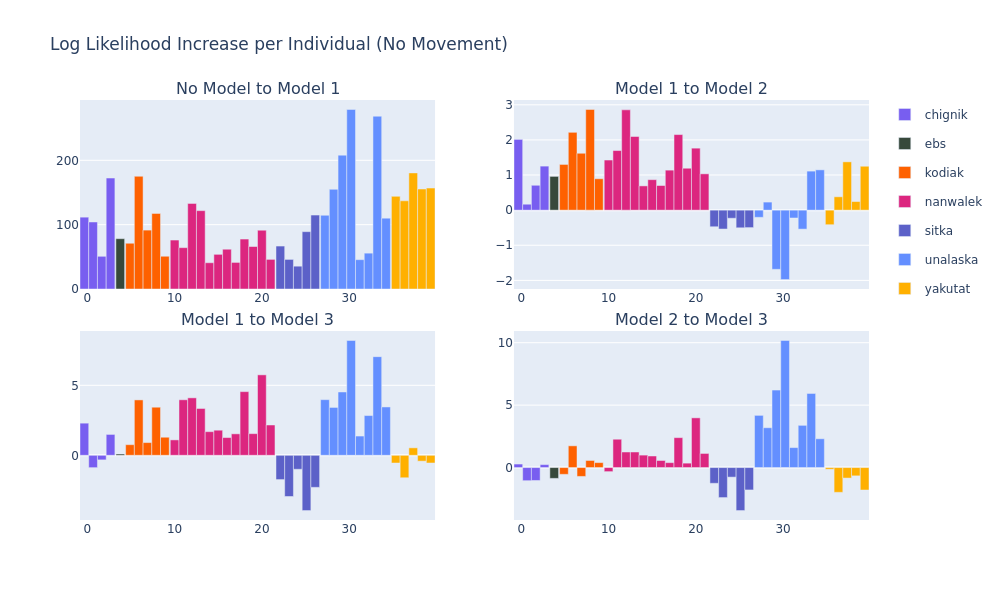
\includegraphics[height=70mm]{figures/ll_increase_no_movement.png}
  \caption{Log likelihood increase (unnormalized) per individual of each model change in cases where the selection involved no movement.}
  \label{fig:ll_increase_no_movement}
\end{figure}

\FloatBarrier

\begin{figure}[h!] 
	\centering
  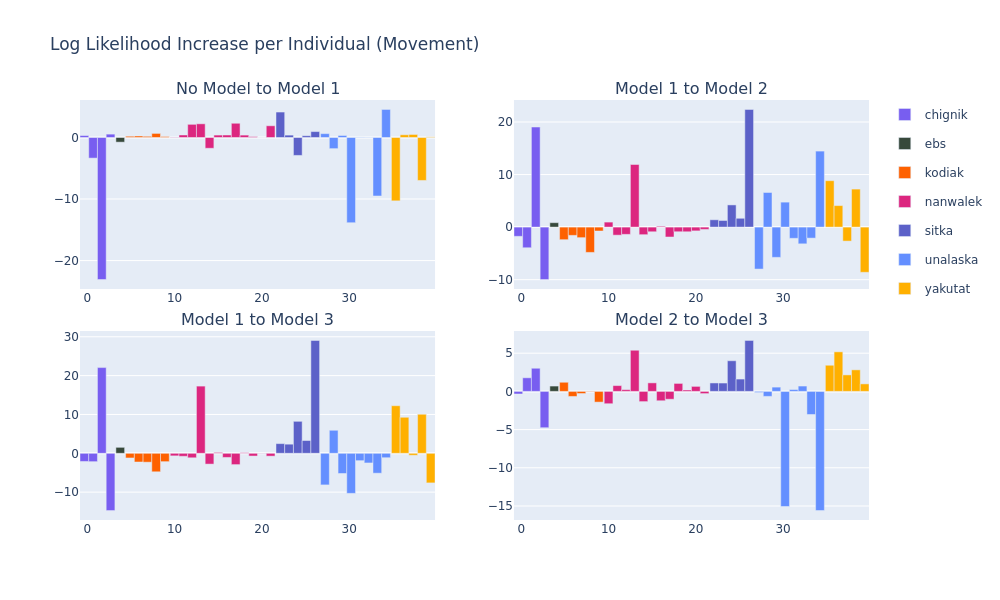
\includegraphics[height=70mm]{figures/ll_increase_movement.png}
  \caption{Log likelihood increase (unnormalized) per individual of each model change in cases where the selection involved movement.}
  \label{fig:ll_increase_movement}
\end{figure}



Figure \ref{fig:ll_increase} shows the unnormalized changes in log likelihood for each individual colored by the region in which they were initially tagged as we go from one model to the next. Figures \ref{fig:ll_increase_no_movement} and \ref{fig:ll_increase_movement} break this down for decisions that resulted in no movement and movement respectively. Only individuals in the validation set were considered.

The appendix contains a series of mapped examples (figures \ref{fig:chignik_map}-\ref{fig:yakutat_map}) from each of these regions (besides EBS) that shows how the log likelihood per decision (when moving) changed in moving from model 1 to model 2 and then from model 2 to model 3. As in the above, only individuals in the validation set were considered.\newline

Finally as much of the behavior seems to be modulated by movement distances (or lack of movement) a summary table of empirical likelihood of movement of a specific distance is given (taken over all individuals). 

\begin{center}
\begin{tabular}{| c | c |}
\hline
Distance Bin (km) & Likelihood of Selection \\
\hline
No Movement & 65.6\% \\
Up to 50km & 32.5\% \\
50km to 100km & 1.9\% \\
\hline

\end{tabular}
\end{center}


\section*{Discussion}

\bibliographystyle{apalike}
\bibliography{reference}
\newpage
\section*{Appendix: Mapped Examples}

\begin{figure}[h!] 
	\centering
  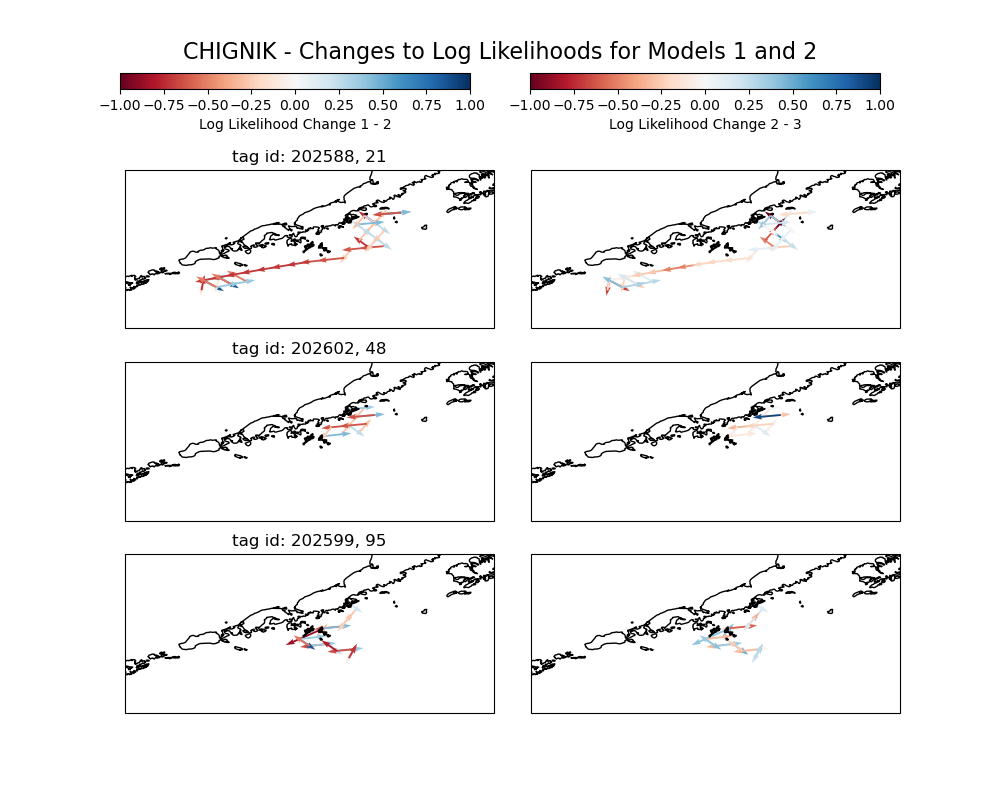
\includegraphics[width=140mm]{figures/chignik_map.png}
  \caption{Log likehood changes per decision - Chignik}
  \label{fig:chignik_map}
\end{figure}

\begin{figure}[h!] 
	\centering
  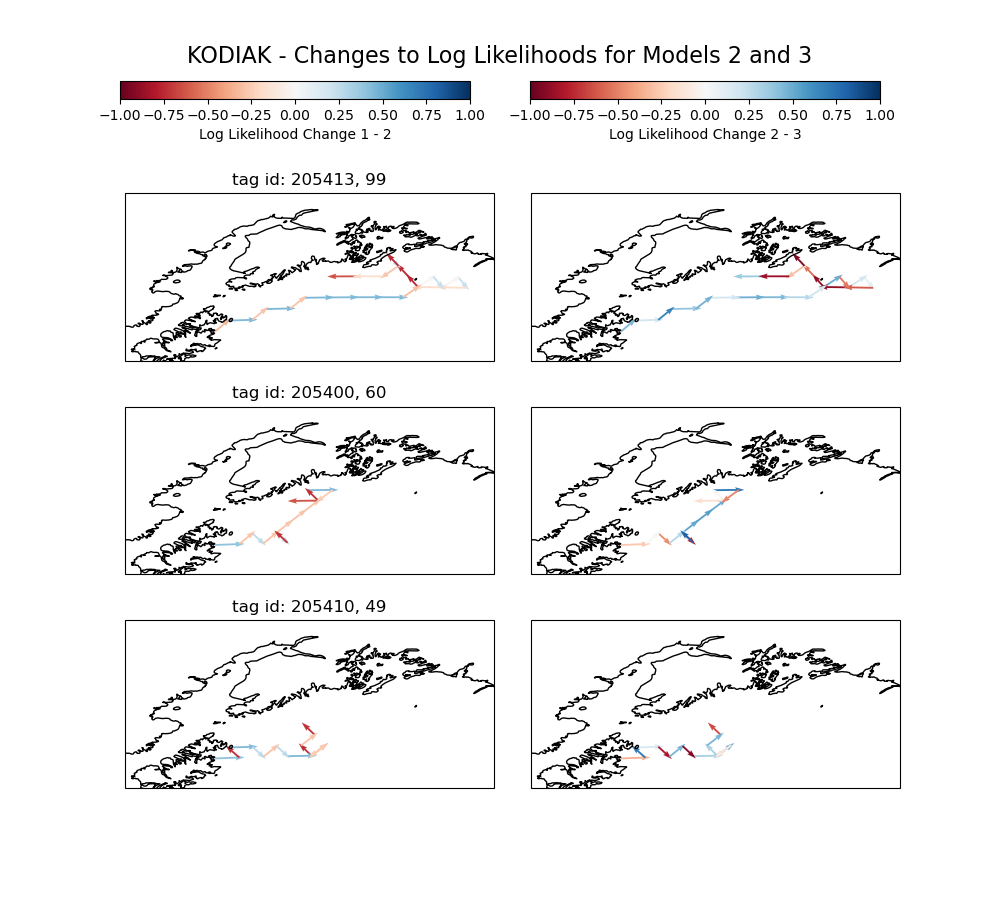
\includegraphics[width=140mm]{figures/kodiak_map.png}
  \caption{Log likehood changes per decision - Kodiak}
  \label{fig:kodiak_map}
\end{figure}

\begin{figure}[h!] 
	\centering
  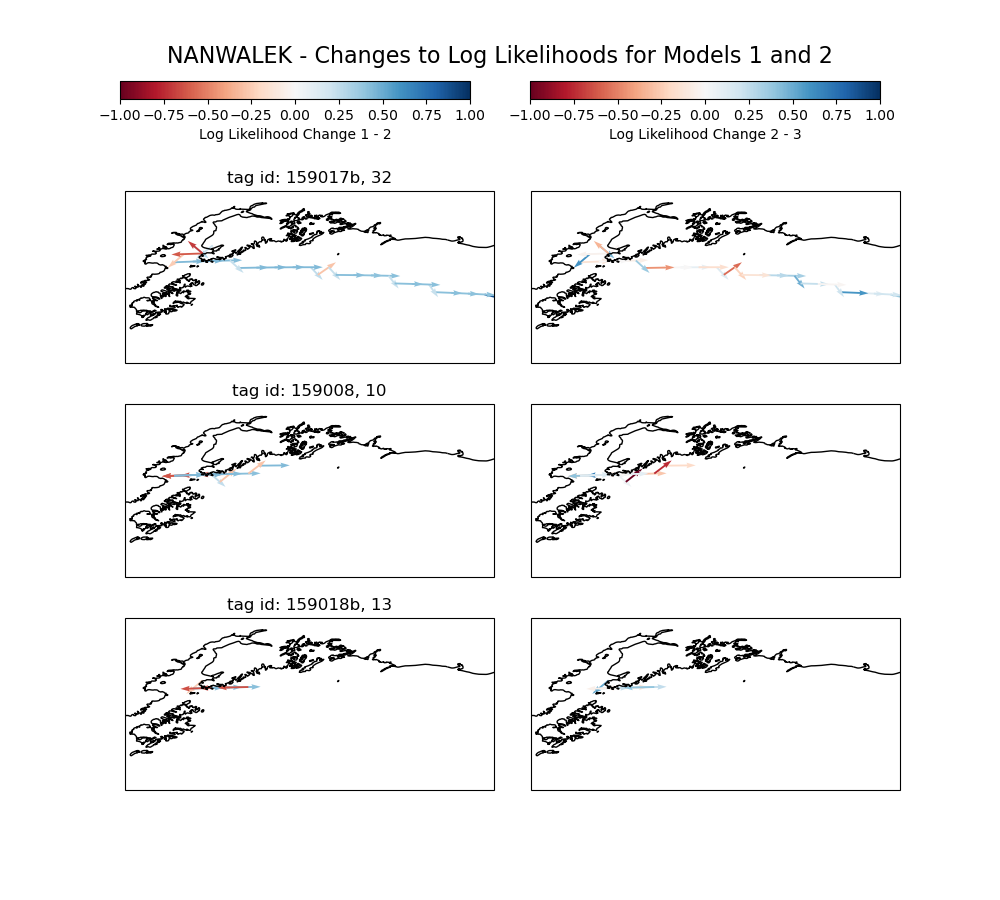
\includegraphics[width=140mm]{figures/nanwalek_map.png}
  \caption{Log likehood changes per decision - Nanwalek}
  \label{fig:nanwalek_map}
\end{figure}

\begin{figure}[h!] 
	\centering
  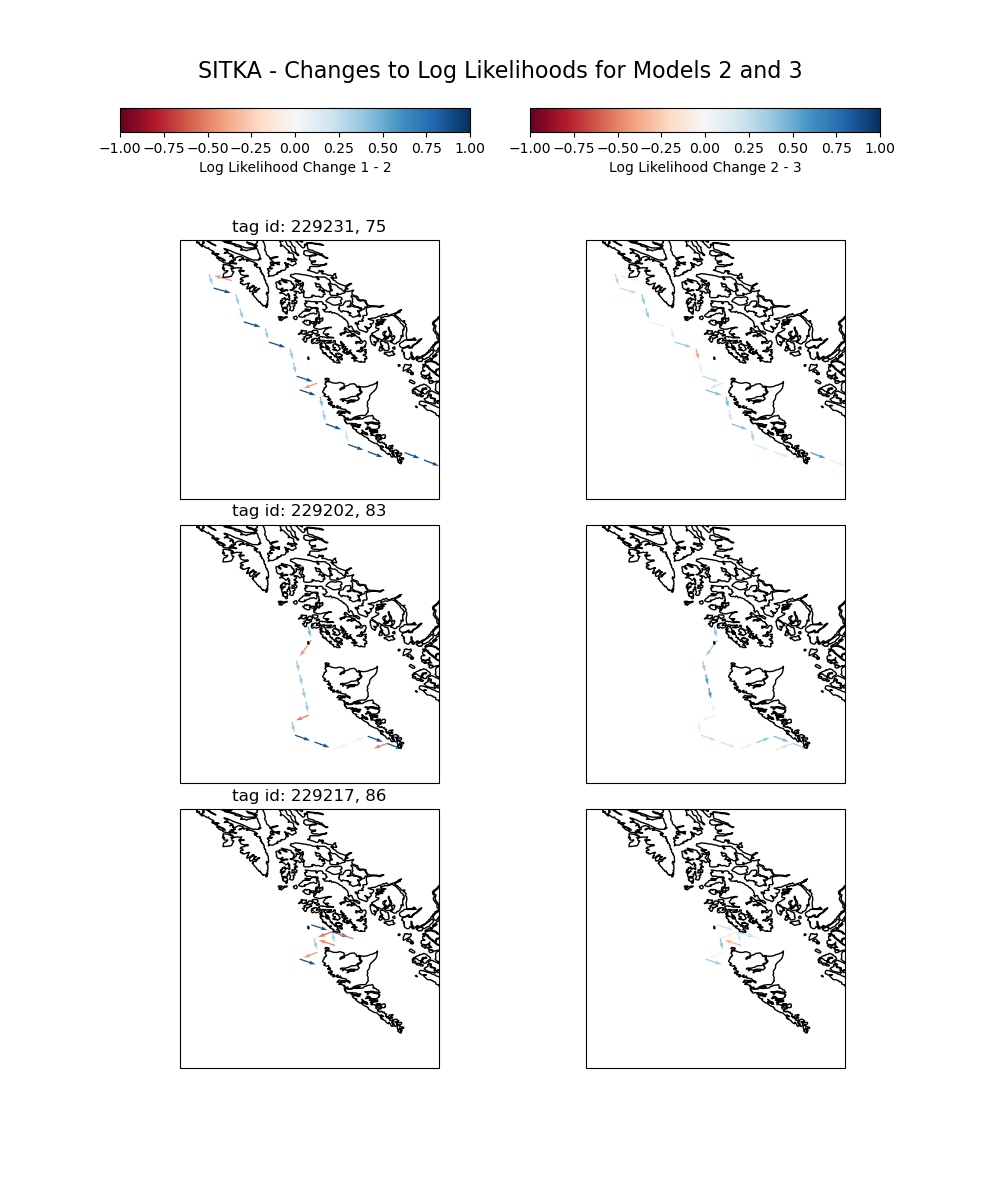
\includegraphics[width=140mm]{figures/sitka_map.png}
  \caption{Log likehood changes per decision - Sitka}
  \label{fig:sitka_map}
\end{figure}

\begin{figure}[h!] 
	\centering
  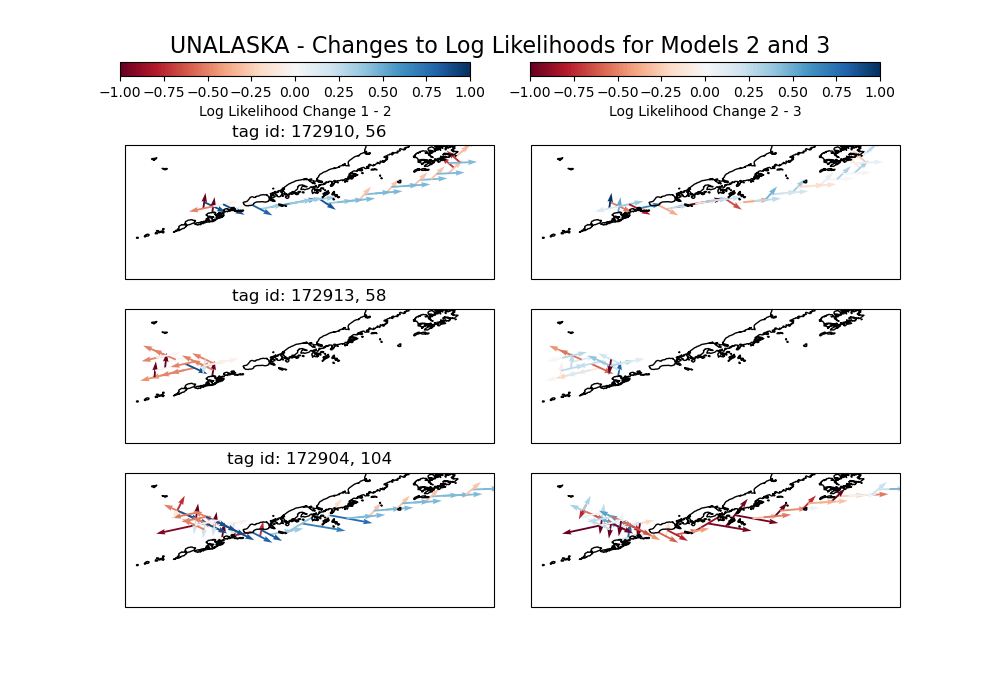
\includegraphics[width=140mm]{figures/unalaska_map.png}
  \caption{Log likehood changes per decision - Unalaska}
  \label{fig:unalaska_map}
\end{figure}

\begin{figure}[h!] 
	\centering
  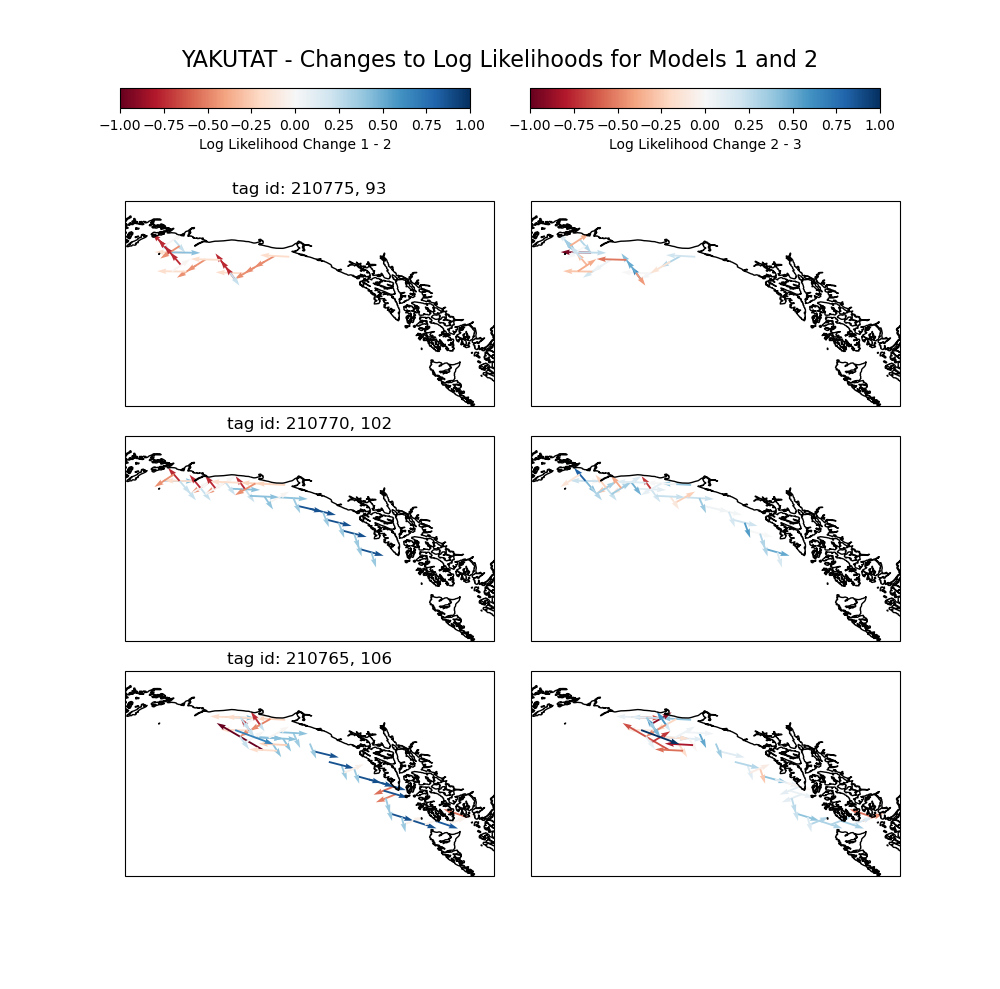
\includegraphics[width=140mm]{figures/yakutat_map.png}
  \caption{Log likehood changes per decision - Yakutat}
  \label{fig:yakutat_map}
\end{figure}

\end{document}